\documentclass{article}
\usepackage{graphicx}
\usepackage{amsmath}
\usepackage{float}
\begin{document}

\title{Top 12 Non-Microcontroller ICs of All Time}
\author{MAHIB}
\date{29/01/2025}
\maketitle

\section{LM555 Timer}
The LM555 is one of the most widely used timer ICs, designed for precision timing applications. It operates in astable, monostable, and bistable modes, making it suitable for oscillators, pulse generators, and delay circuits. The 555 timer is robust, widely available, and still popular in modern electronics.
\begin{figure}[H]
    \centering
    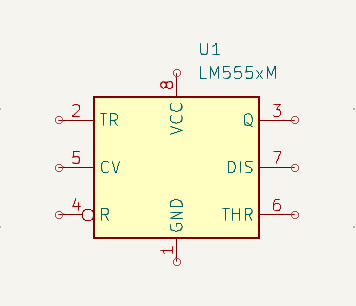
\includegraphics[width=0.5\textwidth]{img/LM555.png}
    \caption{A sample image}
    \label{fig:sample_image}
\end{figure}

\section{LM741 Operational Amplifier}
The LM741 is a general-purpose operational amplifier known for its versatility in analog circuits. It provides high gain and operates with a single or dual power supply. Commonly used in signal conditioning, filtering, and analog computation, the LM741 remains a benchmark for op-amp designs.
\begin{figure}[H]
    \centering
    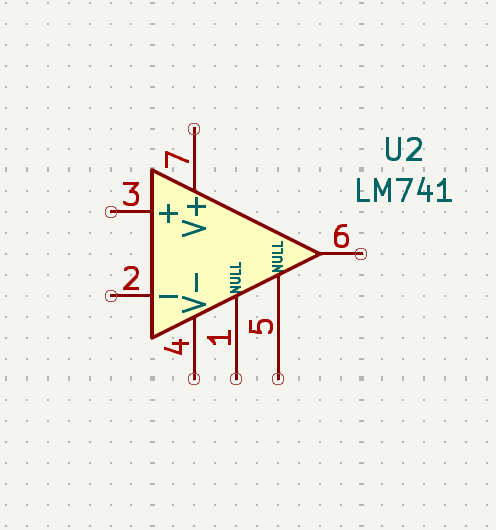
\includegraphics[width=0.5\textwidth]{img/LM741.png}
    \caption{LM741 PinOut}
    \label{fig:LM741}
\end{figure}

\section{LM7805 Voltage Regulator}
The LM7805 is a fixed 5V linear voltage regulator that provides a stable output voltage from a higher input voltage. It is widely used in power supplies for embedded systems, microcontrollers, and various electronic circuits. Its ease of use and reliability make it an industry-standard voltage regulator.
\begin{figure}[H]
    \centering
    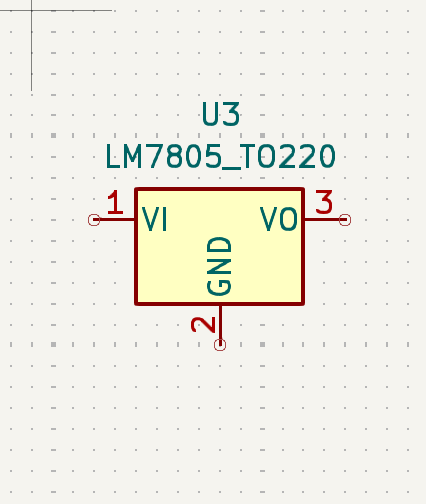
\includegraphics[width=0.5\textwidth]{img/LM7805.png}
    \caption{LM7805 PinOut}
    \label{fig:LM7805}
\end{figure}

\section{ICL8038 Waveform Generator}
The ICL8038 is a precision waveform generator IC capable of producing sine, square, and triangular waveforms with high frequency stability. Used in signal generation, testing equipment, and modulation circuits, it provides low distortion output and is ideal for function generator applications.
\begin{figure}[H]
    \centering
    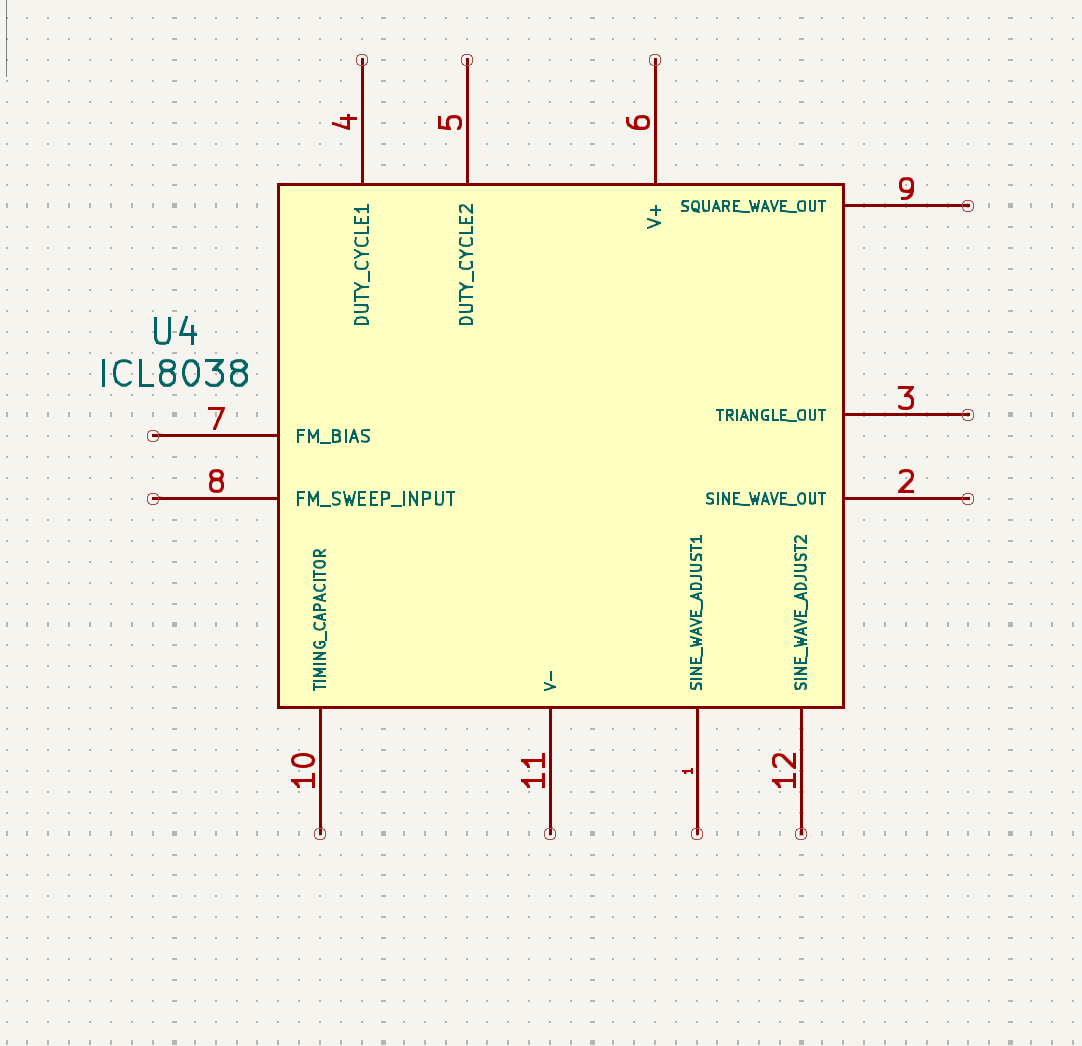
\includegraphics[width=0.5\textwidth]{img/ICL8038.png}
    \caption{ICL8038 PinOut}
    \label{fig:ICL8038}
\end{figure}

\section{TA2020 Audio Amplifier}
The TA2020 is a Class-T digital audio amplifier IC developed by Tripath. It combines the efficiency of Class-D amplifiers with the low distortion of Class-AB amplifiers. Popular in high-fidelity audio applications, it delivers superior audio quality with high efficiency and low power dissipation.
\begin{figure}[H]
    \centering
    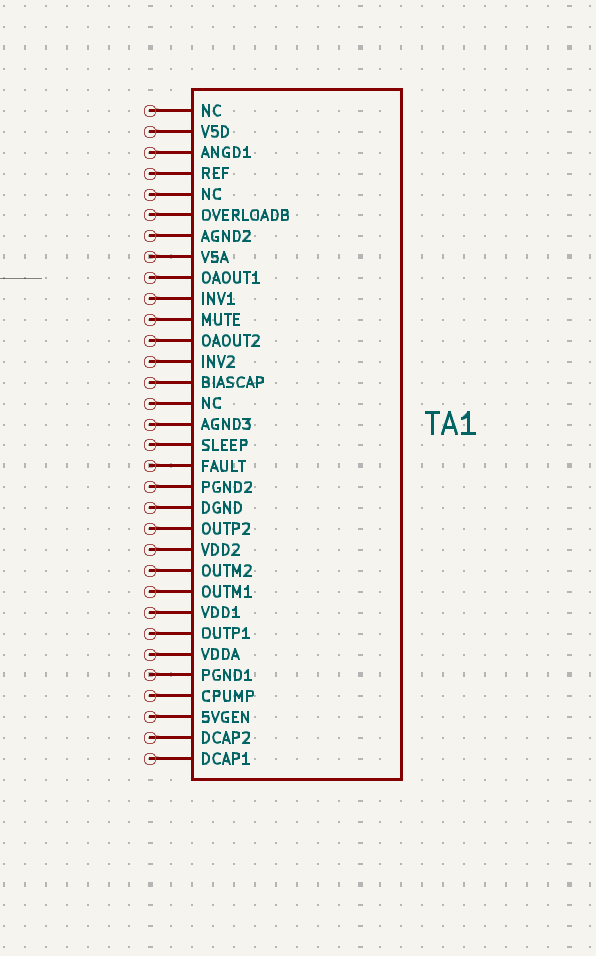
\includegraphics[width=0.5\textwidth]{img/TA2020.png}
    \caption{TA2020 Audio Amplifier PinOut}
    \label{fig:TA2020}
\end{figure}

\section{TL431 Shunt Voltage Regulator}
The TL431 is a programmable shunt voltage regulator widely used in power supply circuits. It provides adjustable voltage regulation with high accuracy, making it useful in switching regulators, battery chargers, and precision voltage references. Its versatility and stability make it a key component in voltage regulation applications.
\begin{figure}[H]
    \centering
    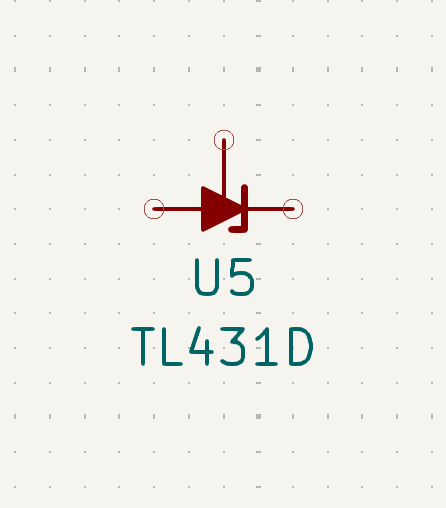
\includegraphics[width=0.5\textwidth]{img/TL431.png}
    \caption{TL431 PinOut}
    \label{fig:TL431}
\end{figure}

\section{CD4007 CMOS Inverter}
The CD4007 is a versatile CMOS IC containing complementary MOSFET pairs. It is commonly used in logic circuits, analog switches, and signal processing applications. Due to its flexible configuration, it serves as a building block for various digital and analog circuits, including inverters and amplifiers.
\begin{figure}[H]
    \centering
    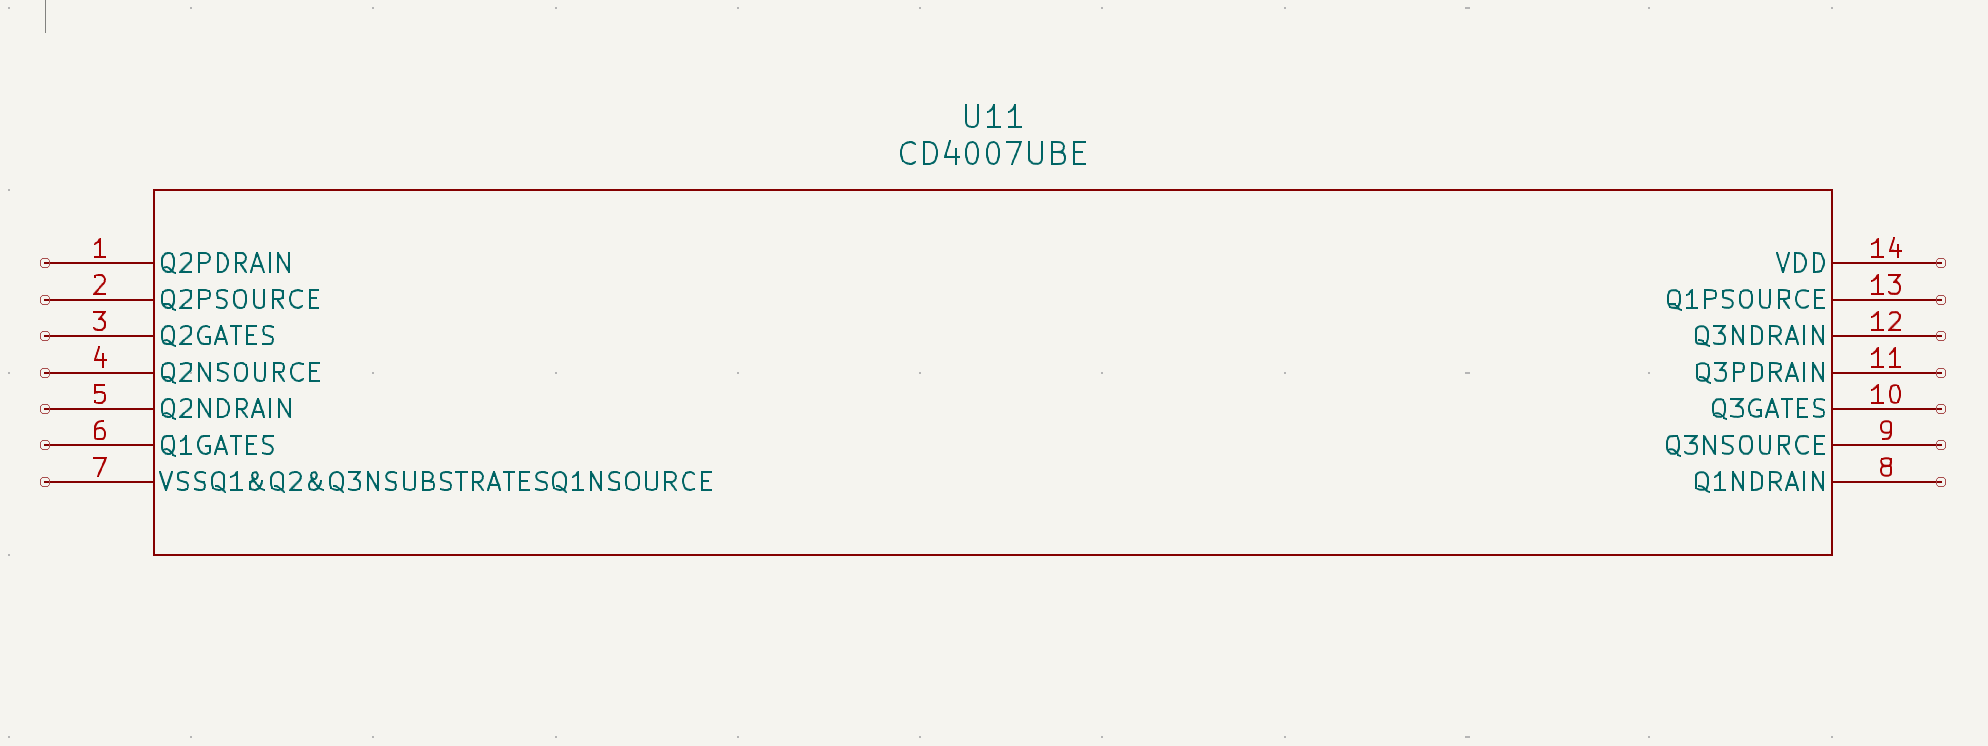
\includegraphics[width=0.5\textwidth]{img/CD4007.png}
    \caption{CD4007 PinOut}
    \label{fig:CD4007}
\end{figure}

\section{7400 Quad NAND Gate}
The 7400 IC is a quad two-input NAND gate from the 7400 TTL logic family. It is fundamental in digital electronics, forming the basis of combinational and sequential logic circuits. NAND gates are universal gates, allowing the construction of any Boolean function with minimal components.
\begin{figure}[H]
    \centering
    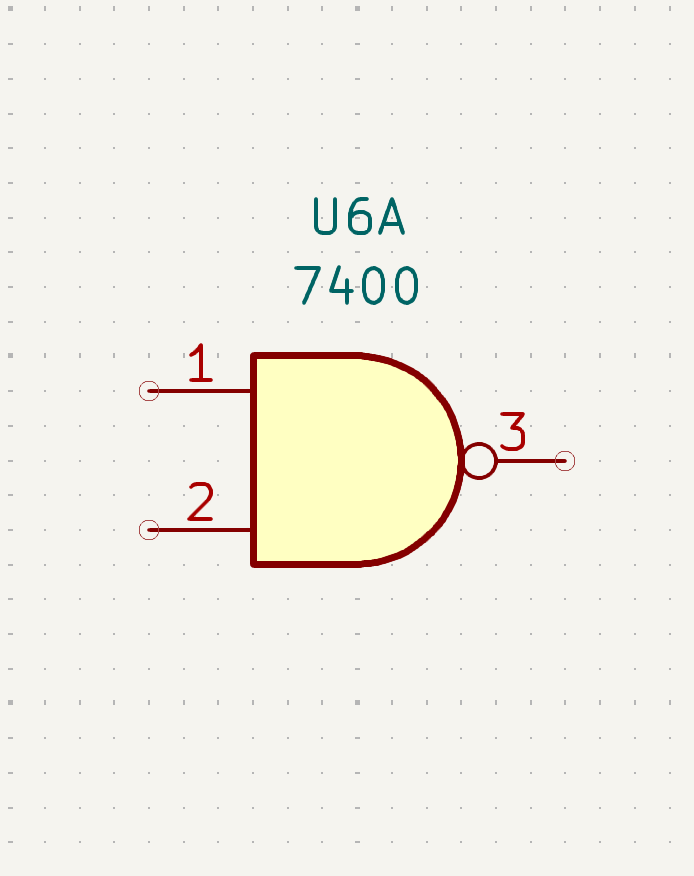
\includegraphics[width=0.5\textwidth]{img/7400.png}
    \caption{7400 PinOut}
    \label{fig:7400}
\end{figure}

\section{LM723 Voltage Regulator}
The LM723 is a versatile linear voltage regulator that supports both high and low voltage applications. It can regulate outputs from 2V to 37V and is used in precision power supplies. It provides adjustable voltage regulation, short-circuit protection, and current limiting, making it highly reliable.
\begin{figure}[H]
    \centering
    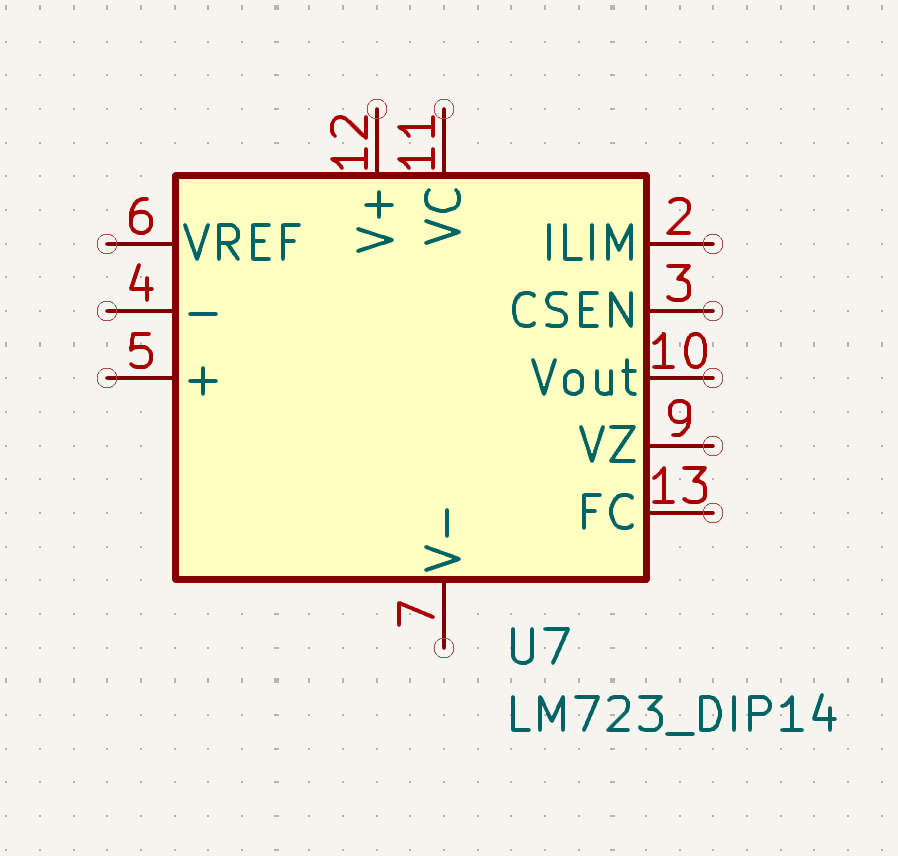
\includegraphics[width=0.5\textwidth]{img/LM723.png}
    \caption{LM723 PinOut}
    \label{fig:LM723}
\end{figure}

\section{LM565 Phase-Locked Loop (PLL)}
The LM565 is a phase-locked loop (PLL) IC used in frequency synthesis, demodulation, and motor speed control applications. It provides stable and precise frequency locking, making it valuable in communication systems, signal processing, and automatic frequency control circuits.
\begin{figure}[H]
    \centering
    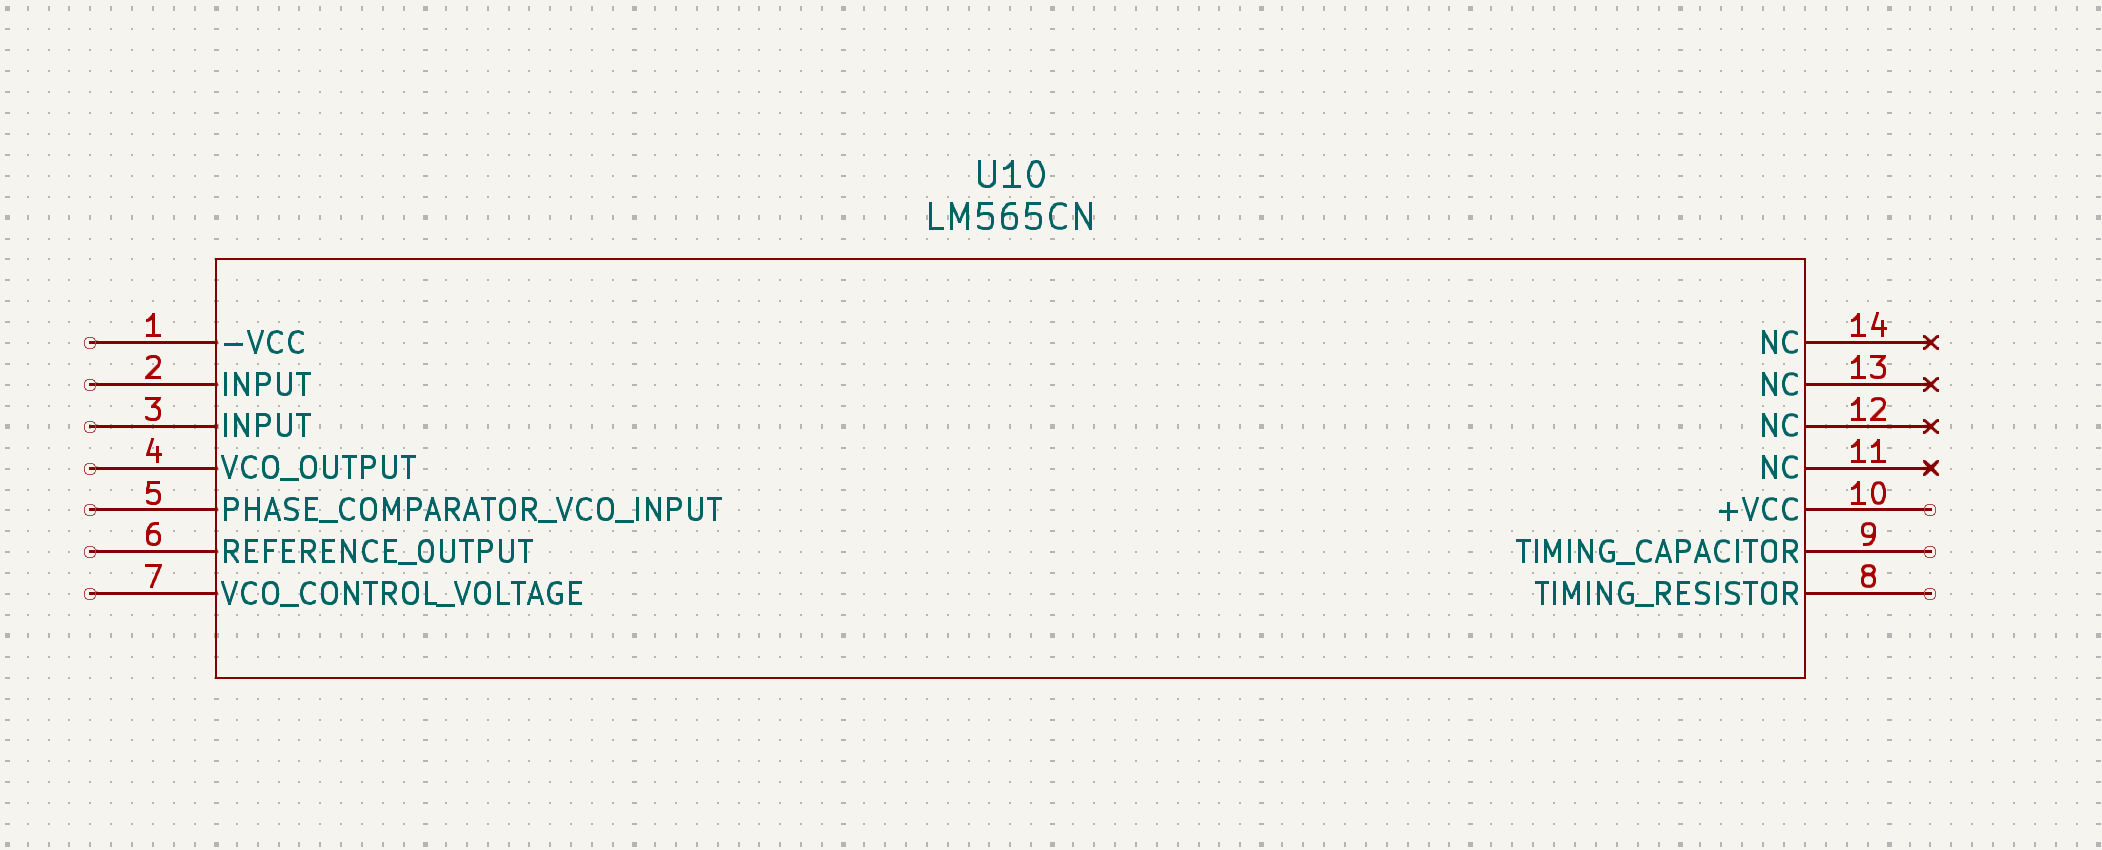
\includegraphics[width=0.5\textwidth]{img/LM565.png}
    \caption{LM565 PinOut}
    \label{fig:LM565}
\end{figure}

\section{LM317 Variable Voltage Regulator}
The LM317 is a 3-pin adjustable voltage regulator that provides output voltages ranging from 1.25V to 37V. It is widely used in power supply applications due to its ease of use and reliable performance. With built-in thermal and overload protection, it remains a popular choice for voltage regulation.
\begin{figure}[H]
    \centering
    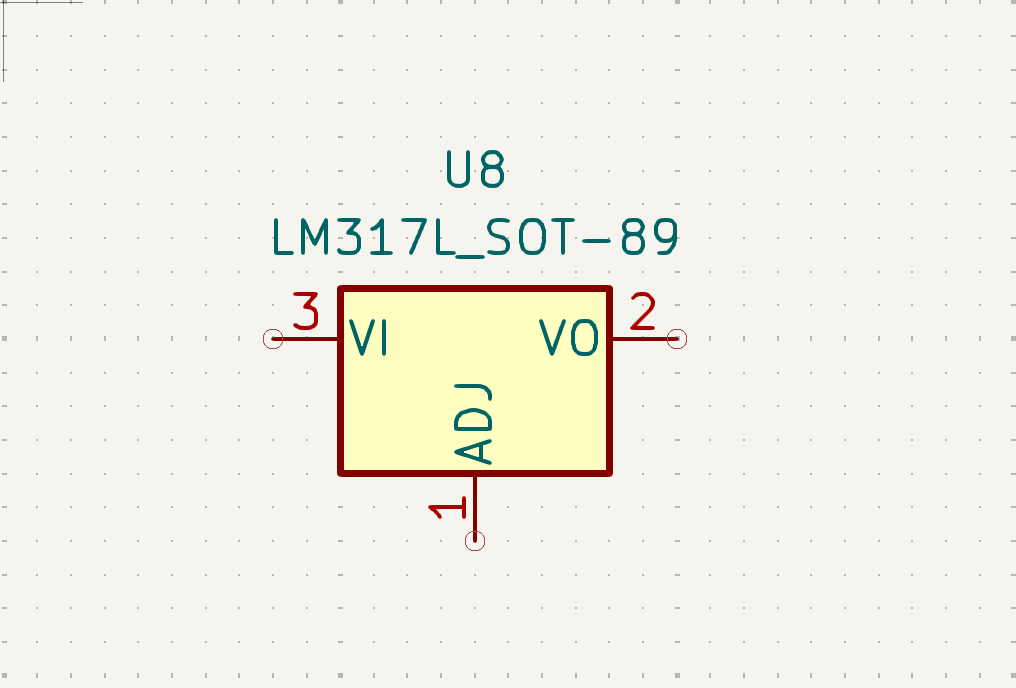
\includegraphics[width=0.5\textwidth]{img/LM317.png}
    \caption{LM317 PinOut}
    \label{fig:LM317}
\end{figure}

\section{ULN2003/2803 Darlington Transistor Array}
The ULN2003 and ULN2803 are high-current Darlington transistor arrays used for driving inductive loads such as relays, stepper motors, and LED displays. They feature built-in clamping diodes for protection, making them ideal for interfacing microcontrollers with high-power loads in industrial and automation applications.
\begin{figure}[H]
    \centering
    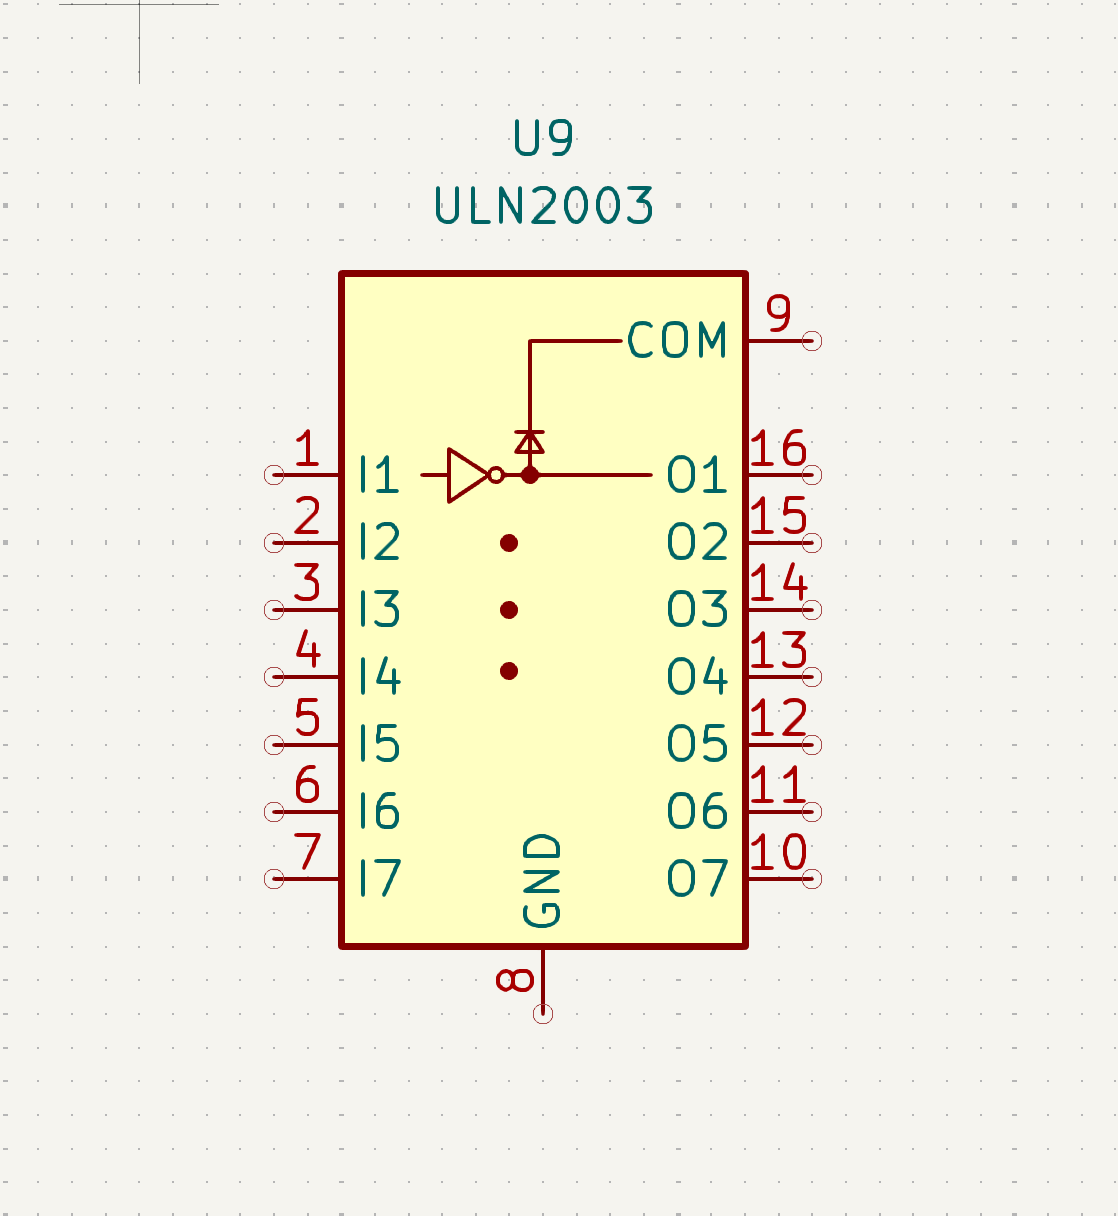
\includegraphics[width=0.5\textwidth]{img/ULN2003.png}
    \caption{ULN2003 PinOut}
    \label{fig:ULN2003}
\end{figure}

\end{document}
